%%%%%%%%%%%%%%%%%%%%%%%%%%%%%%%%%%%%%%%%%%%%%%%%%%%%%%%%%%%%%%%%%%%%%%  
\chapter{Sonstiges}
\label{sec:Sonstiges}
%%%%%%%%%%%%%%%%%%%%%%%%%%%%%%%%%%%%%%%%%%%%%%%%%%%%%%%%%%%%%%%%%%%%%%  


%%%%%%%%%%%%%%%%%%%%%%%%%%%%%
\section{Postergestaltung}
\label{sec:Postergestaltung}

(Beispiele siehe Postertafel des Instituts)

\minisec{Schwerpunkte}
\begin{compactitem}
	\item Kurzvorstellung der Aufgabe
	\item Anschauliche Darstellung des L�sungsweges und wesentlicher Ergebnisse, m�glichst durch Bilder und Tabellen unterst�tzt (kurze Texte, 14 pt / 3mm)
	\item Zusammenfassende Wertung der Ergebnisse und Ausblick auf noch zu l�sende Probleme.
\end{compactitem}

\minisec{Gestaltung}
\begin{compactitem}
	\item Gr��e: 
		\begin{compactitem}
			\item DIN A2-Querformat (59,4 x 42,0 cm), allseitiger Rand 2 cm
	\end{compactitem}
	\item Kopf:
		\begin{compactitem}
			\item �berschrift (Kurzthema), Schriftgr��e: 90 pt, fett (20 mm)
			\item Logo-Block (Schriftgr��e: 18 pt (4 mm) / 14 pt (3 mm):
		\end{compactitem}
\end{compactitem}

\begin{figure}[ht]
	\centering{
		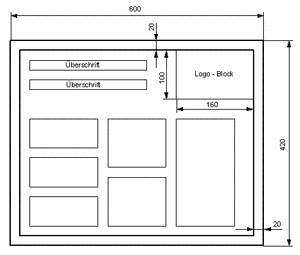
\includegraphics[keepaspectratio, width=9cm]{example_files/RTEmagicC_poster.jpg}
	}
	\label{fig:poster}
	\caption{Gestaltungsrichtlinie des Posters, Ma�e und Abst�nde}
\end{figure}

\minisec{Gestaltung des Logo-Blocks}
Ma�e und Schriftgr��en siehe oben

\begin{figure}[ht]
	\centering{
		
\includegraphics[keepaspectratio, width=9cm]{example_files/RTEmagicC_muster.jpg}
	}
	\label{fig:poster-logo-block}
	\caption{Gestaltungsrichtlinie des Logo-Blocks des Posters}
\end{figure}


%%%%%%%%%%%%%%%%%%%%%%%%%%%%%%%%%%%%%%%%%%%%%%%%%%%%%%
\section{Informationsmittel zur Literaturrecherche}
\label{sec:InformationsmittelZurLiteraturrecherche}

Wegen der st�ndig anwachsenden Zahl von Ver�ffentlichungen ist es angebracht, bei der Literaturrecherche rationelle Methoden anzuwenden.
Daf�r stehen in den wissenschaftlichen Bibliotheken
\begin{compactitem}
	\item S�chsische Landesbibliothek - Staats- und Universit�tsbibliothek (SLUB)
	\item Fachbibliothek Elektrotechnik und Informationstechnik (FBE, DrePunct, Zellescher Weg 17)
\end{compactitem}
Informationsmittel zur Verf�gung.

\begin{table*}[h]
	\centering
		\caption{Kataloge}
		\label{tab:Kataloge}
		\begin{tabular}{lll}%{p{4cm}p{4cm}p{4cm}}
			\toprule
			Bezeichnung & 														& Standort \\
			\midrule
			{\bf Kataloge}		& Alphabetischer Katalog 						& SLUB, FBE \\
        							& Sachkatalog 					 				& SLUB, FBE \\
        							& Dissertationskatalog   						& SLUB, FBE \\
        							& Zeitschriftenkatalog   						& SLUB, FBE \\
        							& Zentralkatalog 				 				& SLUB \\
			\multicolumn{2}{l}{Bibliographien}					 				& SLUB, FBE \\
    			\multicolumn{2}{l}{Firmenschriften/Prospekte/Wirtschaftsliteratur}	& SLUB \\
    			\multicolumn{2}{l}{Normen} 											& SLUB, FBE \\
    			\multicolumn{2}{l}{Dokumentations- und Referatedienste}				& SLUB, FBE \\
    			\multicolumn{2}{l}{Patente}											& SLUB \\ 				
			\bottomrule
		\end{tabular}	
\end{table*}

\minisec{Rechnergest�tzte Recherche-Mittel}
\begin{compactitem}
	\item Rechnergest�tzter Katalog OPAC (Monographie-Bestand der SLUB)
	\item Recherchen in CD-ROM-Datenbanken verschiedener Hersteller (SLUB)
	\item IEEE-Dokumente: Aufs�tze, Tagungsbandbeitr�ge etc. (Volltexte seit 1951 von Uni-IP)
	\item TOC Premier: Zeitschrifteninhaltsverzeichnisse f�hrender Verlage weltweit (Literaturrecherche von Uni-IP)
	\item Datenbank FIZ Technik und Unterdatenbanken: (Literaturrecherche von Uni-IP)
	\item Online-Informationsdienst in kostenpflichtigen Datenbanken (SLUB)
	\item Internet
\end{compactitem}